\documentclass{beamer}
\usepackage{amsmath}
\usepackage{graphicx}
\usepackage{booktabs}
\usepackage{colortbl}

\usetheme{Madrid}
\usecolortheme{default}

\title[Learning to Reason under Off-Policy Guidance]{Learning to Reason under Off-Policy Guidance}
\author{Summary by GitHub Copilot}
\institute{From the paper by Jianhao Yan, Yafu Li, et al.}
\date{\today}

\begin{document}

\begin{frame}
    \titlepage
\end{frame}

\begin{frame}{Outline}
    \tableofcontents
\end{frame}

\section{Motivation: The Limits of On-Policy RLVR}

\begin{frame}{The Problem with On-Policy Learning}
    \begin{itemize}
        \item Reinforcement Learning with Verifiable Rewards (RLVR) has shown success in training Large Reasoning Models (LRMs).
        \item However, these methods are inherently \textbf{on-policy}.
        \item \textbf{Limitation}: Learning is restricted to the model's own outputs. The model can only amplify existing behaviors and struggles to acquire reasoning abilities beyond its initial capabilities.
        \item \textbf{Core Question}: How can we empower models to learn reasoning behaviors that surpass their initial cognitive boundaries?
    \end{itemize}
\end{frame}

\section{LUFFY: The Proposed Framework}

\begin{frame}{LUFFY: An Overview}
    \frametitle{Learning to Reason Under oFF-policY guidance}
    \begin{figure}
        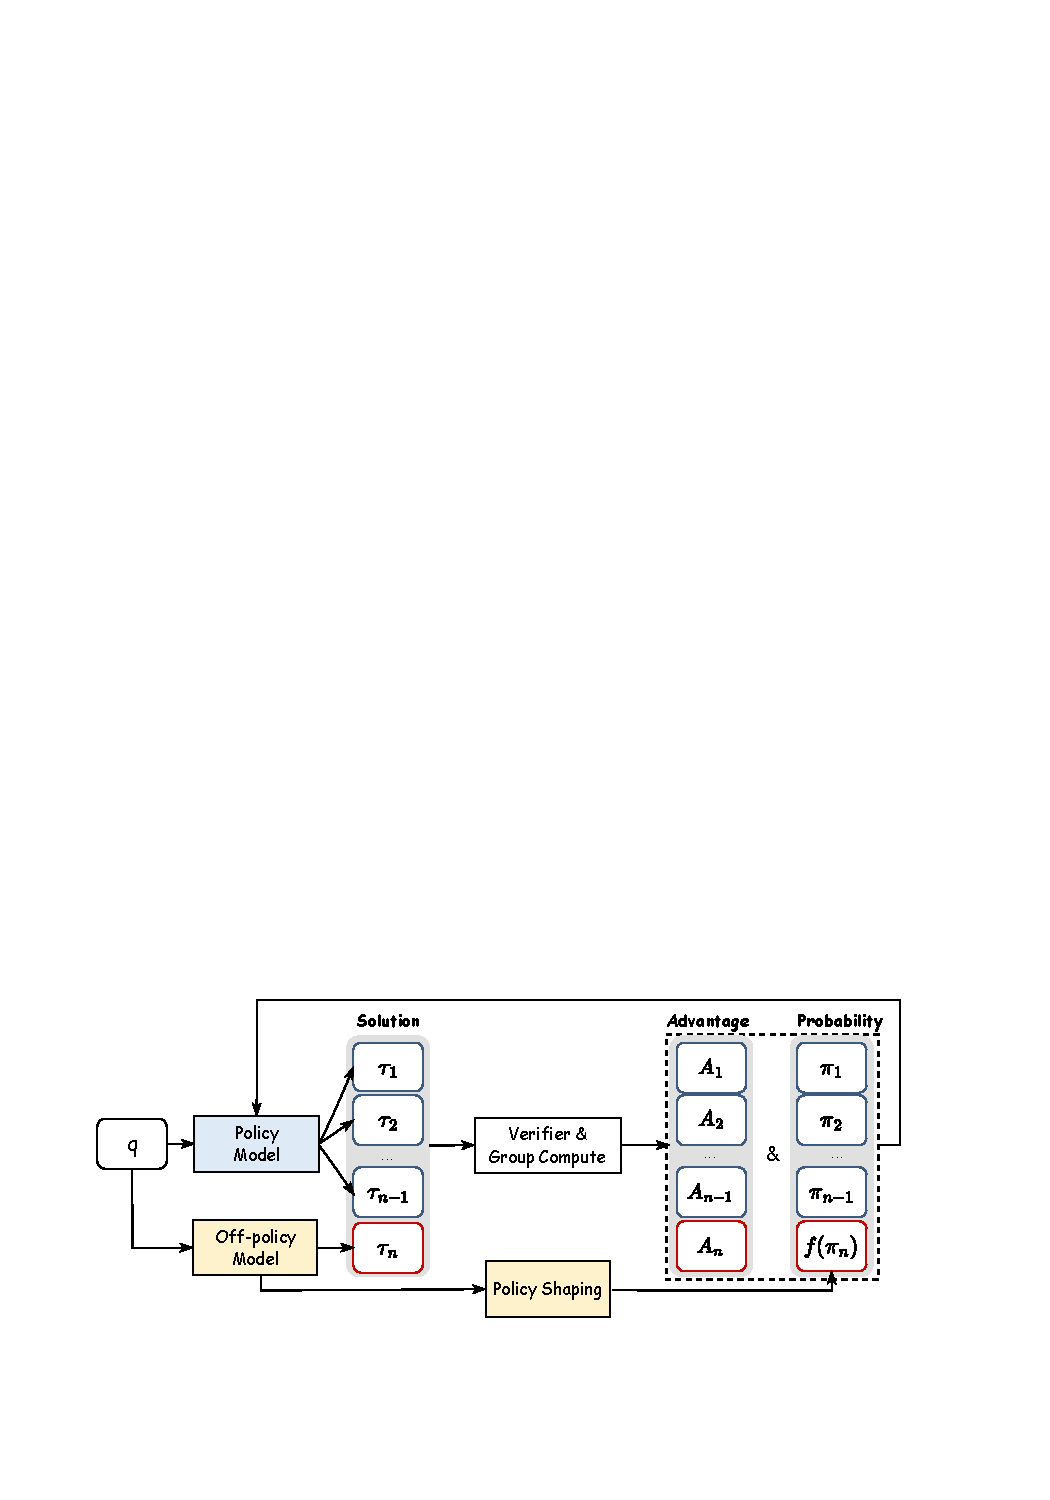
\includegraphics[width=\textwidth]{figs/off-GRPO.v3.drawio.pdf}
        \caption{LUFFY integrates off-policy reasoning traces into RL by combining them with on-policy rollouts, using policy shaping to balance imitation and exploration.}
    \end{figure}
\end{frame}

\subsection{Mixed-Policy GRPO}
\begin{frame}{Mixed-Policy GRPO: Core Idea}
    \begin{itemize}
        \item LUFFY extends Group Relative Policy Optimization (GRPO) by incorporating \textbf{off-policy guidance} (e.g., reasoning traces from a stronger model).
        \item It combines on-policy rollouts ($\mathcal{G}_{\text{on}}$) with off-policy demonstrations ($\mathcal{G}_{\text{off}}$) to compute the advantage $\hat{A}_i$.
        \end{itemize}
        \begin{equation*}
            \hat{A}_i = \frac{R(\tau_i) - \text{mean}(\mathcal{G}_{\text{on}} \cup \mathcal{G}_{\text{off}})}{\text{std}(\mathcal{G}_{\text{on}} \cup \mathcal{G}_{\text{off}})}
        \end{equation*}
    \begin{itemize}
        \item \textbf{Intuition}: The model imitates high-quality off-policy traces when its own attempts fail, but explores on its own when it succeeds. This creates a dynamic balance between imitation and exploration.
    \end{itemize}
\end{frame}

\begin{frame}{Mixed-Policy GRPO: The Objective Function}
    The objective function includes terms for both off-policy and on-policy trajectories.
    \begin{equation*}
    \resizebox{0.9\hsize}{!}{$
        \mathcal{J}_{\text{Mixed}}(\theta) = \frac{1}{Z} (\underbrace{\sum_{j=1}^{N_{\text{off}}} \sum_{t=1}^{|\tau_j|} 
        \text{CLIP}(\hat{r}_{j,t}(\theta, \phi),\hat{A}_j, \epsilon)}_{\text{off-policy objective}}
        + \underbrace{\sum_{i=1}^{N_{\text{on}}} \sum_{t=1}^{|\tau_i|} \text{CLIP}(r_{i,t}(\theta),\hat{A}_i, \epsilon)}_\text{on-policy objective})
    $}
    \end{equation*}
    \begin{itemize}
        \item Importance sampling ratios are used to correct the policy gradient:
        \begin{itemize}
            \item On-policy: $r_{i,t}(\theta) = \frac{\pi_\theta(\tau_{i,t} | \dots)}{\pi_{\theta_{\text{old}}}(\tau_{i,t} | \dots)}$
            \item Off-policy: $\hat{r}_{j,t}(\theta, \phi) = \frac{\pi_{\theta}(\tau_{j,t} | \dots)}{\pi_{\phi}(\tau_{j,t} | \dots)}$
        \end{itemize}
    \end{itemize}
\end{frame}

\subsection{Policy Shaping}
\begin{frame}{The Challenge: Entropy Collapse}
    \begin{itemize}
        \item While Mixed-Policy GRPO works, it can lead to a new problem: \textbf{Entropy Collapse}.
        \item The model converges too quickly, leading to deterministic outputs and reduced exploration.
        \item This happens because the model tends to reinforce off-policy tokens that are already likely under its own policy, ignoring low-probability (but potentially crucial) tokens that represent new reasoning steps.
    \end{itemize}
    \begin{figure}
        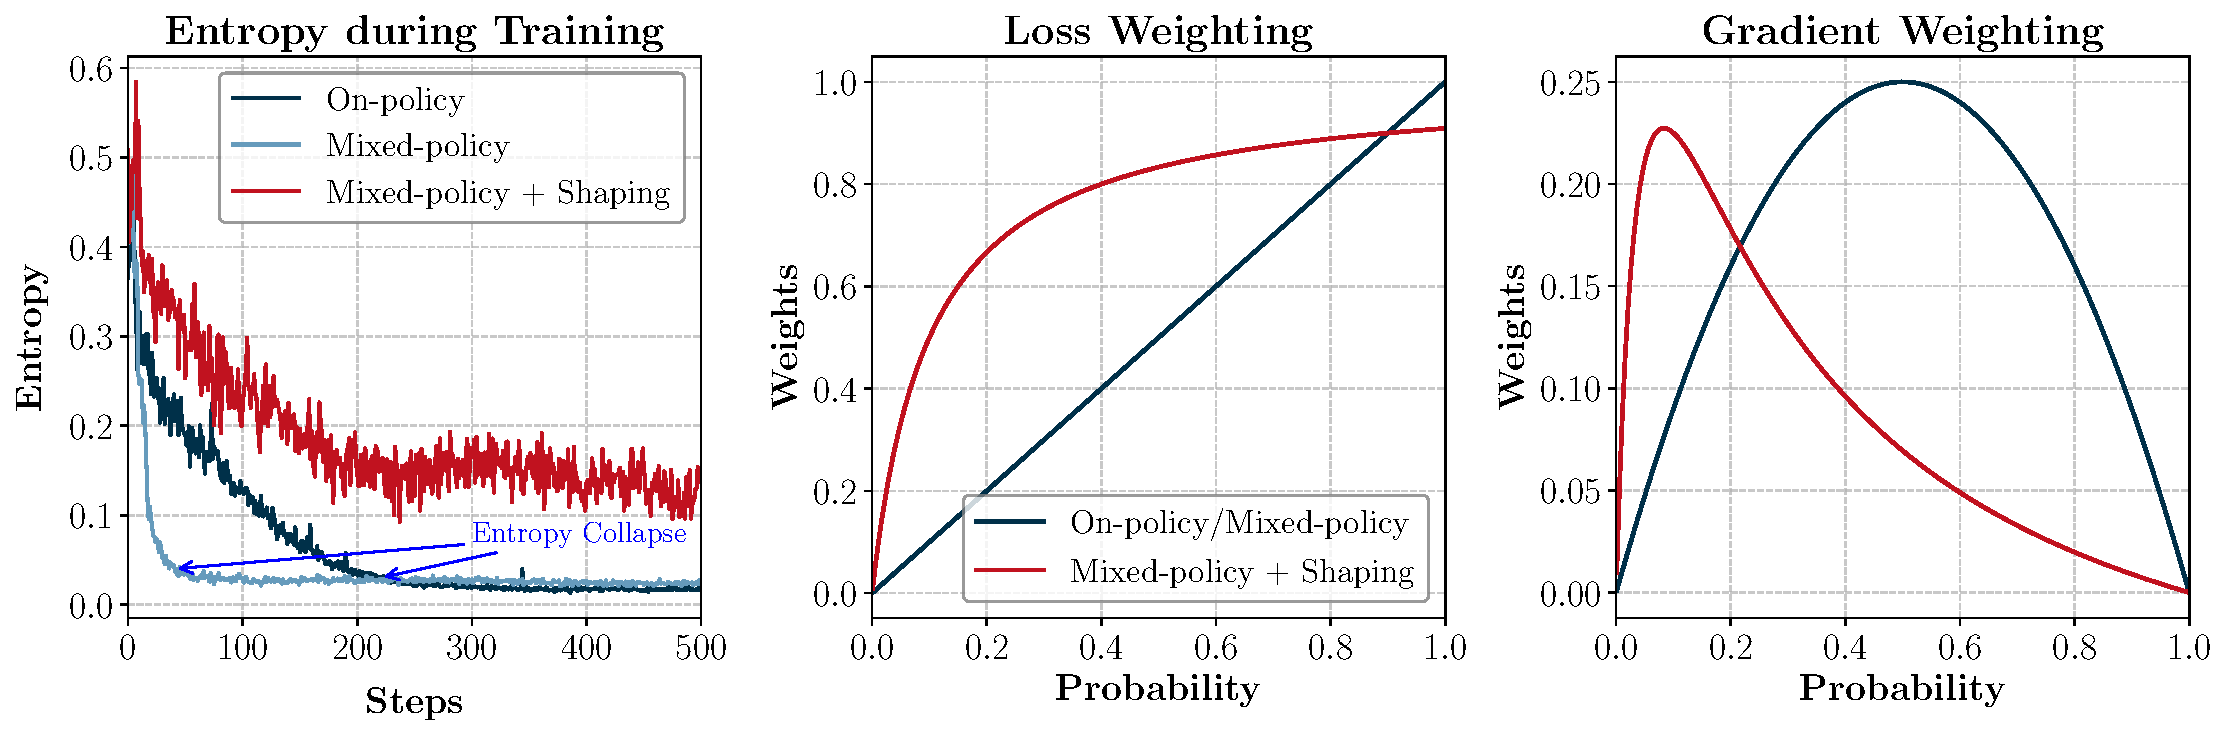
\includegraphics[width=0.7\textwidth]{figs/entropy_func.pdf}
        \caption{Left: Entropy collapses faster in Mixed-Policy GRPO compared to On-Policy RL.}
    \end{figure}
\end{frame}

\begin{frame}{Solution: Policy Shaping}
    \frametitle{Policy Shaping via Regularized Importance Sampling}
    \begin{itemize}
        \item To counter entropy collapse, LUFFY introduces \textbf{policy shaping}.
        \item The idea is to re-weight the gradient of the off-policy distribution to amplify the learning signal for low-probability tokens.
        \item This is done by replacing the off-policy importance sampling ratio $\hat{r}_{j,t}$ with a transformation $f(\hat{r}_{j,t})$.
        \begin{equation*}
            \mathcal{J}_{\text{SHAPING-OFF}}(\theta) \propto \sum_{j=1}^{N_{\text{off}}} \sum_{t=1}^{|\tau_j|} 
            f(\hat{r}_{j,t}(\theta, \phi))\cdot \hat{A}_j
        \end{equation*}
        \item The paper uses the shaping function $f(x) = \frac{x}{x+\gamma}$, which reweights the gradients to assign more importance to low-probability actions.
    \end{itemize}
\end{frame}

\begin{frame}{How Policy Shaping Works}
    \begin{figure}
        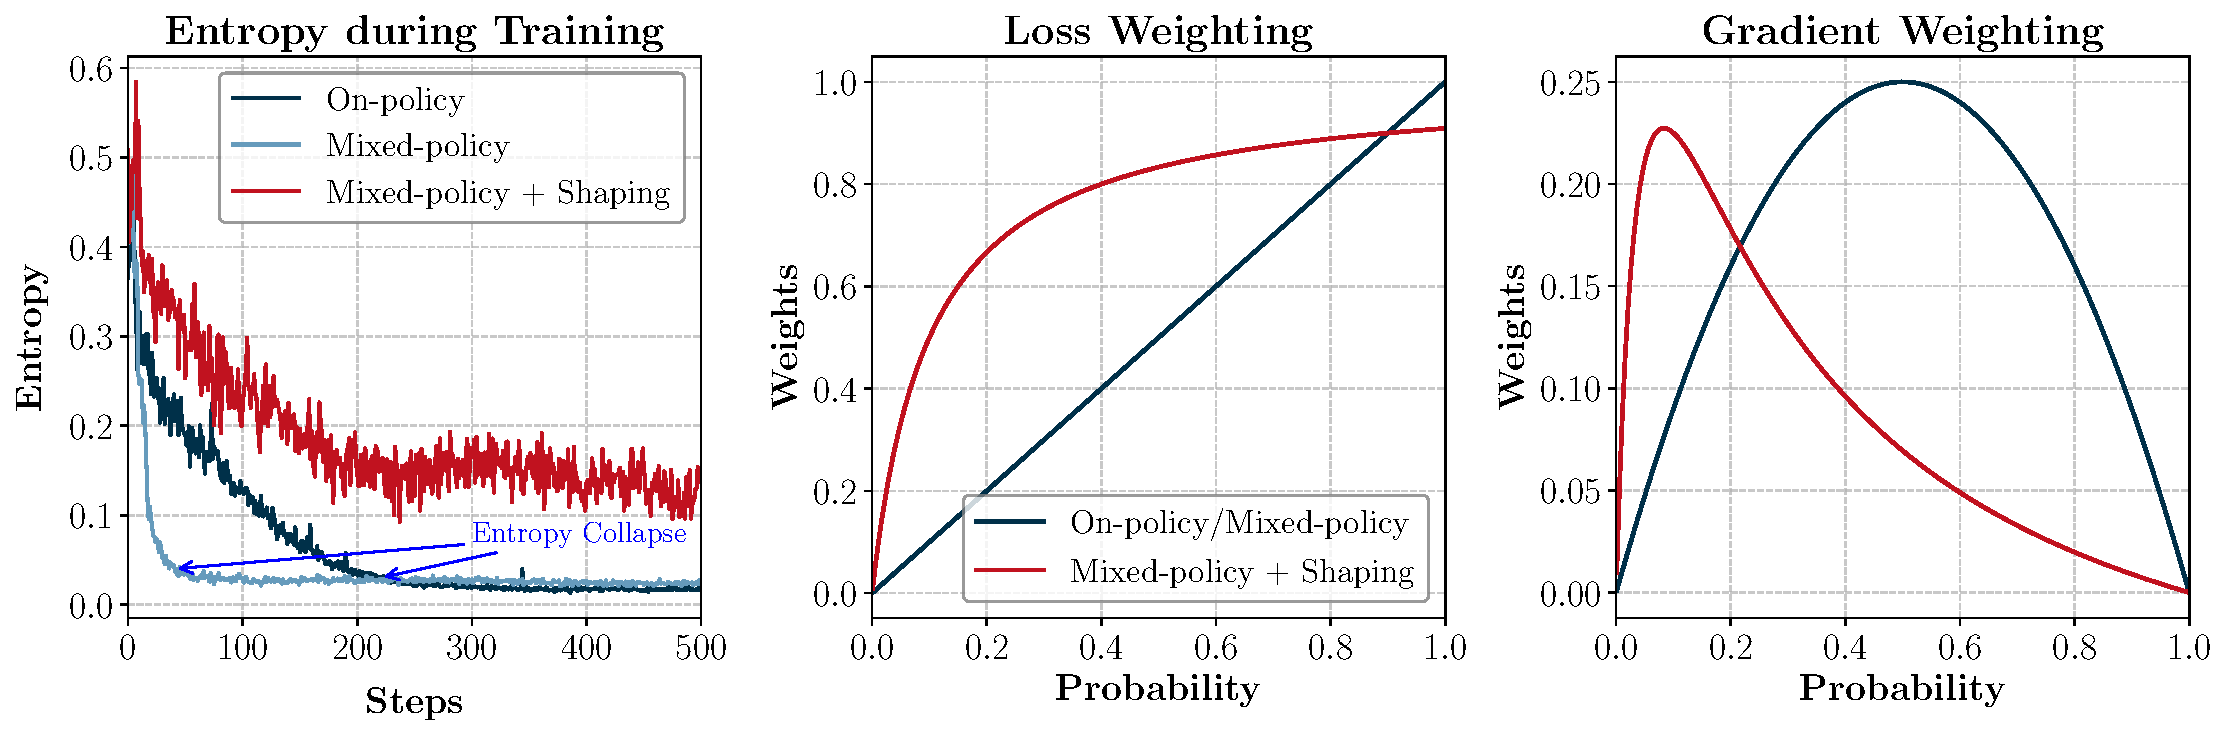
\includegraphics[width=\textwidth]{figs/entropy_func.pdf}
        \caption{Middle: The shaping function $f(x)$ value. Right: The resulting gradient weights are amplified for low-probability actions.}
    \end{figure}
    \begin{itemize}
        \item The derivative of the shaping function, $f'(\pi_\theta)$, acts as a weight on the gradient.
        \item As shown in the figure, this weighting scheme ensures that even when an action's probability $\pi_\theta$ is very low, its gradient receives significant weight.
        \item This encourages the model to continuously explore and learn from unfamiliar but effective actions found in the off-policy traces.
    \end{itemize}
\end{frame}

\section{Conclusion}

\begin{frame}{Algorithmic Summary}
    \begin{itemize}
        \item \textbf{Problem}: On-policy RL is limited by the model's initial knowledge.
        \item \textbf{LUFFY's Solution}: Integrate off-policy guidance.
        \item \textbf{Core Mechanism 1: Mixed-Policy GRPO}
        \begin{itemize}
            \item Dynamically balances imitation (of off-policy traces) and exploration (of on-policy rollouts) by mixing them in the advantage calculation.
        \end{itemize}
        \item \textbf{Core Mechanism 2: Policy Shaping}
        \begin{itemize}
            \item Prevents premature convergence (entropy collapse) by amplifying gradients for low-probability actions in off-policy traces.
            \item This ensures the model learns novel reasoning patterns instead of just reinforcing what it already knows.
        \end{itemize}
    \end{itemize}
\end{frame}

\end{document}
